\documentclass[12pt]{article}
%Gummi|065|=)
\usepackage{amsmath, amsfonts, amssymb}
\usepackage[margin=0.5in]{geometry}
\usepackage{xcolor}
\usepackage{graphicx}
\usepackage{wasysym}

\newcommand{\off}[1]{}
\DeclareMathSizes{20}{30}{20}{18}

\newcommand{\two }{\sqrt[3]{2}}
\newcommand{\four}{\sqrt[3]{4}}
\newcommand{\red}{\begin{tikz}[scale=0.25]
\draw[fill=red, color=red] (0,0)--(1,0)--(1,1)--(0,1)--cycle;\end{tikz}}
\newcommand{\blue}{\begin{tikz}[scale=0.25]
\draw[fill=blue, color=blue] (0,0)--(1,0)--(1,1)--(0,1)--cycle;\end{tikz}}
\newcommand{\green}{\begin{tikz}[scale=0.25]
\draw[fill=green, color=green] (0,0)--(1,0)--(1,1)--(0,1)--cycle;\end{tikz}}

\usepackage{tikz}

\title{Curve Fitting}
\author{John D Mangual}
\date{}
\begin{document}

\fontfamily{qag}\selectfont \fontsize{12.5}{15}\selectfont

\maketitle

\noindent I feel there are ways to do curve-fitting that look up and down the ladder of abstractions.  Let's start with something pretty vanilla: \\ \\
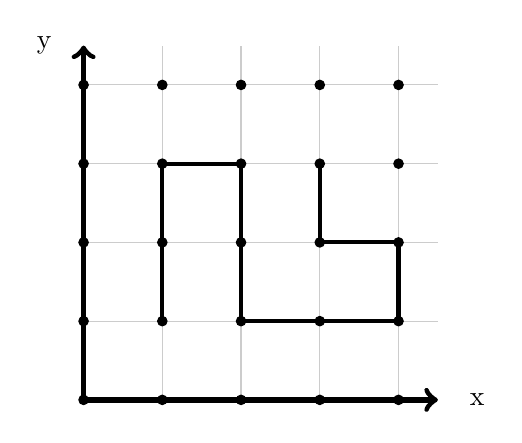
\begin{tikzpicture}

\node at ( 5,0) {x};
\node at (-0.5,4.5) {y};

\foreach \a in {0,...,4}{ 
	\draw[color=black!20!white] (\a,0)--(\a,4.5);
	\draw[color=black!20!white] (0,\a)--(4.5,\a);
 }

\draw[line width=2, ->] (0,0)--(4.5,0);
\draw[line width=2, ->] (0,0)--(0,4.5);

\foreach \a in {0,...,4}{
\foreach \x in {0,...,4}{
			\draw[fill=black] (\a,\x) circle (0.06);
	 }
}


\draw[line width=1.5] (1,1)--(1,2)--(1,3)--(2,3)--(2,1)--(4,1)--(4,2)--(3,2)--(3,3);
\end{tikzpicture} \\ 
Can we draw a curve that passes through all these points?  There are two strategies to try to hook around this many constraints:
\begin{itemize}
\item Lagrange Interpolation
\item Bezier Curves
\end{itemize} 
And maybe it depends on the type of constraint problem you are trying to solve: 
\begin{itemize}
\item passing through points
\item weaving arround points
\end{itemize}
I think one way to motivate a theory is to start with a problem you want to solve.\footnote{Other times, theories comes out of the box, complete. I think such theories are unusuable, or they leave from for input from you and me.  A comeback from that camp could be, ``John, why are you so obsessed with this particular problem?"  And I don't have any good reason.  Just because.  Sometimes about me, and the time and place makes me interested.  And I could be wrong!} We like to brag about how good we are at weaving around constraints.  How bad can we be?  Let $f: [0,1] \to \mathbb{R}$ be a real-valued function:
$$ f(x) = \left\{  \begin{array}{cc} 1 & x \notin \mathbb{Q}  \\ 
0 & x \in \mathbb{Q} \end{array} \right. $$
Then we can ask what the integral is between $0$ and $1$.  Overwhelmingly, the answer should be:
$$ \int_0^1 f(x) \, dx = 1 \times \Big|\{ x \notin \mathbb{Q}  \}\cap [0,1]\Big| + 0 \times \Big|\{ x \in \mathbb{Q}  \}\cap [0,1]\Big| =  1 $$
Relatively innocent-functions like these are sufficient Riemann integration.  I reasoned there are vastly more irrational numbers than rational numbers.


\newpage

\noindent This turns out to be one of the worse functions around, because it looks like $\mathbf{1}$ but isn't:
$$ f(x) \approx \mathbf{1} \quad\text{therefore}\quad \int f \approx \int \mathbf{1} $$
If I recall, we placed intervals around every single fraction $\frac{a}{b} \in \mathbb{Q}$ we get an upper estimate for how large this integral could be, and that upper estimate $ \to 0$.   \\ \\
How to deal with a function that often looks like $f(x) \equiv 1$ but isn't?\footnote{
One set of problems that plagued me was if we had two competing definition of  limit, maybe one returns a number and the other does not.  If we have two limiting procedures $1$ and $2$, maybe: 
$$ \big[ \lim \big]_1 \; a_n = A \quad\text{implies}\quad \big[ \lim \big]_2 \; a_n = A$$
Most of the time we don't really care how the limit procedure is defined.  Who cares really?
$$ N \gg 1 \quad \text{implies}\quad a_N \approx A$$
and the impliciation looks self-evident and most people won't question it.  The only reason we remember the exception is because that particular conversation went on record.} \\ 
\includegraphics{farey-01.png} \\
Here is a plot if we add all of the pure tones at all frequencies $\frac{a}{b}$ with $0 < a < b < 10$.  Theoretically we have found:
$$ \frac{1}{28} \sum_{0 < a < b < 10} e^{2\pi i \frac{a}{b} t} \approx \frac{1}{ c\, N^2 }  \sum_{0 < a < b < N} e^{2\pi i \frac{a}{b} t}
= \left\{ \begin{array}{cc}  1 & \text{if }t = 0 \\ 0 & \text{if }t \neq 0\end{array} \right.  $$
The constant in front is an oversimplification.  The odds of two numbers being relatively primes is a famous one:
$$ \phi(1) + \phi(2) + \dots + \phi(N) = \# \{ (a,b) : a < b \text{ and } \mathrm{gcd}(a,b)=1 \} \approx \frac{2}{\zeta(2)^2} $$
Analysis is the branch of math where we account for all the uses of the $\approx$  symbol.  What if I told you the function we just charted is $\approx {\color{blue}\mathbf{0}}$ ?

\newpage

\noindent When I read someone else's paper, a lot of my surprise stems from the author suggesting there is enough from in function space for something (very unlikely) to occur.  Let's make a little problem set: \\ \\
\# \textbf{1} Show constant function on the rational numbers integrates to zero:
$$ \int_{[0,1]} \mathbf{1}_{\mathbb{Q}} = 0 $$ 
\# \textbf{2} Find a curve that weaves around the obstacle course on page one:\\ \\
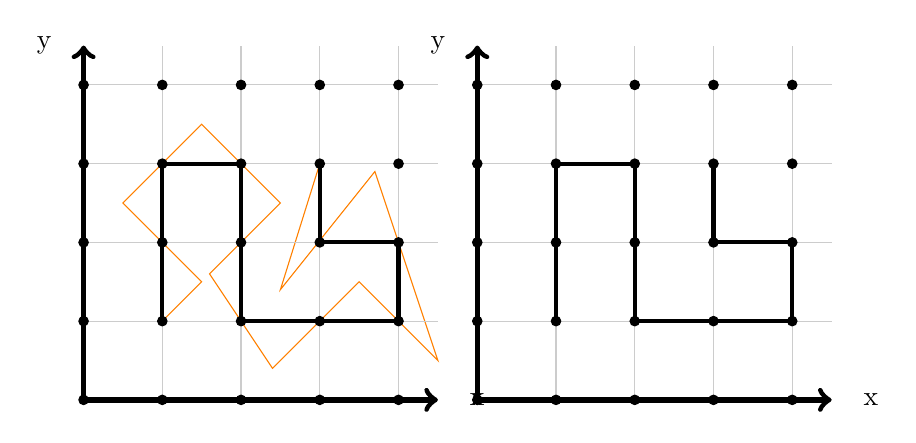
\begin{tikzpicture}

\begin{scope}

\node at ( 5,0) {x};
\node at (-0.5,4.5) {y};

\draw[color=red!50!yellow] (1, 1)--(1.5,1.5)--(0.5,2.5)--(1.5,3.5)--(2.5,2.5)--(1.6,1.6)--(2.4,0.4)
--(3.5,1.5)--(4.5,0.5)--(3.7,2.9)--(2.5,1.4)--(3,3);

\foreach \a in {0,...,4}{ 
	\draw[color=black!20!white] (\a,0)--(\a,4.5);
	\draw[color=black!20!white] (0,\a)--(4.5,\a);
 }

\draw[line width=2, ->] (0,0)--(4.5,0);
\draw[line width=2, ->] (0,0)--(0,4.5);

\foreach \a in {0,...,4}{
\foreach \x in {0,...,4}{
			\draw[fill=black] (\a,\x) circle (0.06);
	 }
}


\draw[line width=1.5] (1,1)--(1,2)--(1,3)--(2,3)--(2,1)--(4,1)--(4,2)--(3,2)--(3,3);



\end{scope}

\begin{scope}[xshift=5cm]

\node at ( 5,0) {x};
\node at (-0.5,4.5) {y};

\foreach \a in {0,...,4}{ 
	\draw[color=black!20!white] (\a,0)--(\a,4.5);
	\draw[color=black!20!white] (0,\a)--(4.5,\a);
 }

\draw[line width=2, ->] (0,0)--(4.5,0);
\draw[line width=2, ->] (0,0)--(0,4.5);

\foreach \a in {0,...,4}{
\foreach \x in {0,...,4}{
			\draw[fill=black] (\a,\x) circle (0.06);
	 }
}


\draw[line width=1.5] (1,1)--(1,2)--(1,3)--(2,3)--(2,1)--(4,1)--(4,2)--(3,2)--(3,3);

\end{scope}

\end{tikzpicture} 
With a pencil it's always possible to draw a curve that passes through all the dots.
Our challenge is to find an equation that passes through all the loops.  This is not so obvious it can always be done. \\ \\
\# \textbf{3} While I am remembering that my other example was going to be, we are going to solve the Prime Number Theorem.  
$$ \Lambda(n) = \left\{ \begin{array}{cl} \log p & \text{if }n=p \\ \\
0 & \text{not prime}\end{array} \right. $$
The prime number says that the density of primes is roughly $ \frac{1}{\text{\# digits}} $ it can also be phrased as:
$$ \sum_{n \leq x} \Lambda(n)  = x + o(x) $$
where $o(x)$ is a really small, unpredictible number\footnote{if you looked at my other projects, a great question to ask would be ``how small", and ``how unpredictible".  We could ask even though $o(x)$ is a small number, maybe it is bigger than $1$ or $5$ or $100$.} This won't be a review of number theory.  Just ironing out one or two parts in a previous discussion.  It's pretty hard. \\ \\
\# \textbf{4} Look at a real paper.  There are one or two short papers of Bourgain that I try to get through from time to time.\footnote{He does not write in a very forgiving way, and occasionally it's so bad, we may as well try to write the step ourselves.}
$$ f(t) = \sum_{|x|, |y|, |z| < N} e^{2\pi i t \; (x^2 + y^2 - \sqrt{2} z^2)} $$ 
This is my favorite way to cause trouble and I get the sense this is the recommended way to start.  A sense that comes from nowhere. .
 \\ \\

\newpage

\noindent All good project start from raw ingredients and tell a story.\footnote{On day I got a textbook ``Methods in Mathematical Physics (Vol 1)"  The book is in German so maybe that's why it was so cheap; it is available in English.  These math-for-phyisicists textbooks are pretty dull.  This is the middle of the 20th century and Math and Physics, which you'd assume were related had taken very different paths.  Mathematicians were tired of calculations and instead proposed to build a world entirely of abstrct principles.  Physicists needed to build things and used math whenever they needed it, or fabricated their own\dots Courant-Hilbert managed to write a textbook that assembles hundreds of unrelated techniques into a pretty-good story.  And it's still the story in the modern literature, more or less.}  For me pictures form an engine that start projects.  Or it could be a memory or something that happened. \\
\includegraphics[width=5in]{node-01.png} \\ 
These pictures of the vibrating nodes (``notes" \quarternote\twonotes\quarternote\, ) of a square drum were made are before computer graphics (the textbook was written in the 1930s). Drafting and technical drawing (without computers) seems like stupid and arcane technical skill, but our ability to make things of good quality is constrained by this.  Maybe the textbooks fail to make the case. \\
\includegraphics[width=5in]{node-02.png} \\ 
Generating these curves with computer is not so easy.  The equation for both of these is:
$$ f(x,y) = 0 $$
for some judiciously chosen function $f$.  In the case of the square we can try sines and cosines:
$$ f(x,y) = \sum_{m, n \in \mathbb{Z}} a_{m,n} \sin m x \sin n y$$
Maybe I need to include cosines as well.  Different variations.  Why stop at two?  Maybe I can get \textit{every possible pattern} using a level-set of bunch of sine and cosine. \\ \\Additionally, even when we have the equation, solving $f(x,y) = 0$ is not very realistic, maybe solving $f(x,y) < \epsilon$ where $\epsilon =  10^{-3}$ or $10^{-6}$ or however small you are intereted in.  And this becomes an algorithms problem. \\ \\
In the process I may have mixed up two kinds of problems:
\begin{itemize}
\item Drawing the curve (maybe with Bezier curves)
\item Finding a function with reasonable level set (maybe with Lagrange Interpolation)
\end{itemize}
I think they're almost the same but after reading Wikipedia I might be wrong.  When I started off in number theory, there are all these cute averaging statements, such as:
$$  \frac{1}{r_3(n)}\sum_{x^2 + y^2 + z^2 = n} \phi(x,y,z) \ll n^{-1/28} $$
All of these theorems rest on the interpolation results I'm trying to explore here\dots and perhaps all of these number theory problems are sources of ill-behaved functions I am outlining.  \\ \\
All the papers I have seen resort to horrible complicated rearrangements that deserve a better explanation.  

\newpage

\noindent \# \textbf{1} Starting small, let's show that $ \int \mathbf{1}_\mathbb{Q} = 0 $.  The rational numbers are dense but form a set of measure zero.
\begin{itemize}
\item $\overline{\mathbb{Q}}= \mathbb{R}$
\item $\mu(\mathbb{Q}) = 0$
\end{itemize}
You could take for granted that you can always find a fraction close enough to your number 
$$ 47\% = \frac{47}{100} \approx \frac{12}{25} $$
\textbf{12 in 25} sounds pretty good instead of \textbf{47 in 100}.  Maybe one is more persuasive than the other.\footnote{Here we use a tiny bit of projective space $\frac{a}{b} = [a:b] = \mathbb{Q}P^1$ and maybe even a tiny bit of the Galois cohomology of the field $\mathbb{Q}$.  That is my theory what all these $H^1$'s are doing there. }  Even though we say $\mathbb{Q}$ is dense in $\mathbb{R}$, finding any fraction is easy, finding a really good fraction can be some work.  If $\alpha \notin \mathbb{Q}$: 
$$ \exists \, p,q \text{ such that }  \bigg| \frac{p}{q} - \alpha \bigg| < \frac{1}{q^2} $$
Therefore density misses other more refined statements we could make about $\overline{\mathbb{Q}}$. \\ \\
Let's walk through a few sample arguments.  How did I first learn that $\mathbb{Q}$  is a set of measure zero?  This was self-evident to Stein.  A point has measure zero, there are countably many fractions, and therefore $\mathbb{Q}$ has measure zero.
$$ \mu (\{ pt\}) = 0 \text{ and } 
\mu(\mathbb{Q}) \leq \bigcup_{\frac{a}{b} \in \mathbb{Q}} 
\mu(\big\{ | x - \frac{a}{b} | < \frac{\epsilon}{2^k} \big\} ) = 
\epsilon \sum \frac{1}{2^k} = \epsilon \to 0$$
If we index the fractions one by one we can get some kind of geometric series.
$$ (\frac{a_1}{b_1}, \frac{1}{2}) \to 
 (\frac{a_2}{b_2}, \frac{1}{2^2}) \to 
  (\frac{a_3}{b_3}, \frac{1}{2^3}) \to 
   (\frac{a_4}{b_4}, \frac{1}{2^4}) \to \dots 
    (\frac{a_k}{b_k}, \frac{1}{2^k}) \to \dots  $$
There are several enuerations of the fractions we can use, such as the Farey Fractions or the Calkin-Wilf tree or the Stern-Brocot Tree.  The textbook says \textbf{any} enumeration of fractions. Personally, I drew a picture: \\ 
\includegraphics[width=3in]{farey-02.png}

\newpage

\noindent The Calkin-Wilf tree (Wikipedia) \\
\includegraphics[width=3in]{farey-03.png} \\ \\
The Stern-Brocot tree \\ 
\includegraphics[width=3in]{farey-04.png} \\ \\
I really needed to make the countability of the rationals in a tangible, almost deadpan kind of way.  Even there is some research you can do:
\begin{itemize}
\item Carlo Carminati, Giulio Tiozzo \textbf{A canonical thickening of Q and the dynamics of continued fractions} \texttt{arXiv:1004.3790}
\end{itemize}
I have to look to see if there is more.  But now we can appreciate how abstract real analysis can be: we are taking inventory of something infinitely complex and we're just saying it has been done.

\newpage

\noindent Flipping through my old Real Anaysis textbook I found some gems.\footnote{At my school, real analysis at the level of Lebesgue Theory was taught to 3rd year undergraduates who were pretty serious about math. I failed it.  And passed the second time with a B.  These days I almost agree with their assessment because I look at the textbook and still don't really get it.}  I can't look at this picture and not see Dehn's theorem, that if the length and the width are rational, then every single rectangle must have rational length and width.\\ 
\includegraphics[width=3in]{stein-01.png}
\includegraphics[width=4.5in]{stein-02.png} \\ 
I could have spent an entire semester drawing ever more complicated shapes and putting rectangles on them. \\

\includegraphics[width=3in, angle=-90, origin=c]{pavage-01.jpg}\hspace{1in}
\includegraphics[width=3in, angle=-90, origin=c]{pavage-02.jpg}

\begin{thebibliography}{}

\item Richard Courant, David Hilbert.  \textbf{Methoden der mathematischen Physik} (Satz I) Springer, 1937. 

\item Elias Stein, Rami Shakarchi.   \textbf{Analysis III: Real Analysis - Measure Theory, Integration and Hilbert Space }(Princeton Lectures in Analysis) Princeton University Press, 2004.


\end{thebibliography}

\newpage

\noindent \# \textbf{3} There are two approaches I can think of two the prime number theorem that should be written:
\begin{itemize}
\item Real Analysis
\item Ergodicity of the Horocycle Flow
\end{itemize}
and I can put this up here, because if someone beats me to it, I will gladly take their existing argument simplify it and settle for the worse constant.  \\ \\
The starting point is a bit arbitrary, an artifact of how we have developed and do arithmetic over the centuries\dots just the way you and me do:
$$ \Lambda(n) = \left\{ \begin{array}{cl} \log p & \text{if }n=p \\ \\
0 & \text{not prime}\end{array} \right. $$
The prime number says that the density of primes is roughly $ \frac{1}{\text{\# digits}} $ it can also be phrased as:
$$ \sum_{n \leq x} \Lambda(n)  = x + o(x) $$
With a little bit of work, this function can be charted, just like any other. 
We'd like to be able to say the derivative of the second equation is the first one:
$$ \frac{d}{dx} \sum_{n \leq x} \Lambda(n)  = \frac{d}{dx}  \big( x + o(x) \big) = 1 + o(1)  \quad\text{but}\quad \frac{d}{dx} o(x) \stackrel{?}{=} o(1)$$
So our instinct -- mine at least -- really falls apart on this problem.  Unfortunately, I can try to get other instinct and it might look weird, but at least it's more accurate.  For one thing: the line is not prefectly straight: \\
\includegraphics[width=3.5in]{farey-06.png}\hfill
\includegraphics[width=3.5in]{farey-05.png}\\
This took several years to state the problem in a visual way that I felt comforatble with.  It exists in the literature.  Always after you find it, suddently the paper is right there:
\begin{itemize}
\item Don Zagier \textbf{The First Million Prime Numbers}\footnote{http://people.mpim-bonn.mpg.de/zagier/files/doi/10.1007/BF03039306/fulltext.pdf}
\end{itemize}
I really want to drive the point home, how decidedly not straigth these lines are. \\
\includegraphics[width=7.5in]{farey-07.png} \\ 
The prime number theorem is important because there are many other statements that I care about that are equivalent to PNT, so that it has become a sort of ``gatekeeper" for me.  And I can't exactly say I've overcome, but we have a reasonable shot of pinning the last details here: \dots \; \dots \; \dots \\ \\
For now I'm an a hurry I'll state some variants of Prime Number Theorem.  
\begin{itemize}
\item the angle of a prime number in $\mathbb{Z}[i]$ is equidistriuted as $p \gg 1$.  This one doesn't look like PNT at all, it starts from noticing that $5 = 2^2 + 1^2$ but $7 \neq \square + \square$. 
\item the Sato-Tate conjecture
\item the Chebotarev Density Theorem
\end{itemize}
Despite their profound modernity, all of these are slightly old fashioned.  Here I tend to check the most recent arXiv articles to see what the latest conjecture is.\footnote{And experts in other fields are not always sure where the frontier is.  You and I should feel free to settle here, or if you know a lot, to take a brand new position! Here's one:
\begin{itemize}
\item Kaisa Matom\"{a}ki, Maksym Radziwi\l\l, Terence Tao \textbf{An averaged form of Chowla's conjecture} \texttt{ arXiv:1503.05121}
\end{itemize}
The time is certainly approaching!
} \\ \\
I think by the 1920's, 30's and 40's I started to find really good, convincing proofs of PNT.  Parts of it were still being settled the 80's and 90's and up to now.  I heard the version I am about to give, has really bad constants.  \\ \\
If we wanted to we could sequester the Prime Number Theorem to five very basic pages:
\begin{itemize}
\item Don Zagier \textbf{On Newman's Short Proof of the Prime Number Theorem}  American Mahtematical Monthly (1997)
\end{itemize}


\newpage

\noindent Like I said won't spend much time on this. A lot has changed since the 1950's.  I worked out a few solutions in a Starbucks.  Just a summary\footnote{I was surprised to learn from the barista that cold brew coffee was not the same as I coffee.  I had one of each.} \\ \\ 
Buzzwords like ``resurgence" and ``regularization" do not exist yet.  Instead, the textbook proposes a clever use of the Laplace transform:
$$ f(x) = \sum_{n=1}^\infty \frac{\big(\Lambda(n)-1\big)e^{-nx}}{1 - e^{-nx}} $$
Why could this series be solve our problem or natural from number theory? The weight:
$$ \frac{ e^{-nx}}{1 - e^{-nx}} \approx \left\{
\begin{array}{cc} 
\frac{1}{nx} & x \to 0 \\ \\
e^{-nx} & x \gg 1 \end{array}
 \right. \text{ with turning point at } n \approx \frac{1}{x}$$
Using an intelligent choice of filters we'd like to make an approximation, an engineer migth not question it.  A mathematicians could be scared of (rather faint) signals that might change the result:
$$ f(x) = \sum_{n=1}^\infty \frac{\big(\Lambda(n)-1\big)e^{-nx}}{1 - e^{-nx}} \approx 
\frac{1}{x} \sum_{n < \frac{1}{x}} \frac{\Lambda(n)-1}{n}$$
So if we reason this function divergece a certain way, maybe we can collect our result about the primes.  Here are other ways to look at $f$:
$$ f(x) = \int_0^\infty \frac{te^{-xt}}{1 - e^{-xt}} \;d \Bigg[ \sum_{n \leq x} \frac{\Lambda(n)-1}{n}\Bigg] $$
This is a \textbf{Riemann-Stieltjes} integral, which is why I drew the \textbf{spike train} on the previous page.  The measure is no longer $dx$  instead it is 
$$ d \Bigg[ \sum_{n \leq x} \frac{\Lambda(n)-1}{n}\Bigg] = 
\left\{ \begin{array}{cl}
 0 & x \notin \mathbb{Z} \\ \\
 \frac{\Lambda(n)-1}{n}  & x=n \in \mathbb{Z}  \end{array}\right. $$ 
measuring all the places where this function jumps.  And we are convolving this spike train against the generator of the Bernoulli polynomials:
$$ g(x,t) = \frac{te^{-xt}}{1 - e^{-xt}}  \text{ vs } \frac{te^{xt}}{e^t - 1} = \sum_{n=0}^\infty B_n(x) \frac{t^n}{n!} $$
At least, they resemble each other.  Here's another awy to look at $f$
$$ f(x) = \sum_{n=1}^\infty \sum_{m=1}^\infty \{ \Lambda(n)-1 \} e^{-mnx} = 
\sum_{n=1}^\infty \left[ \sum_{d|n} \big(\Lambda(d)-1\big) \right] e^{-nx}$$
He calls it Lambert summation but we can also call it M\"{o}bius transformation.  So there's a way to pass between the van Mangoldt function $\Lambda$ and the just plain $\log$ function.  

\newpage

\noindent Just have that $\log = \Lambda \ast 1$ or $\Lambda = \log \ast \mu $ where $\mu$ is the \textbf{M\"{o}bius} function.   Depending on which source you look, we can prove that:
$$ f(x) \sim -\frac{2\gamma}{x} $$
why is that a solution, though?  ``Abelian" and ``Tauberian" theorems are rather heavy tools, that either blow-up elementary calculations into deeper ones, or extract results that are buried in infinite series.  \\ \\
Norbert Weiner solves the theorem in a few pages (plus 20 or 30 pages devoted to proving the Tauberian theorem)
$$ \sum_{m=1}^\infty (\log m ) x^m = \dots = \sum_{n=1}^\infty \Lambda (n) \frac{x^n}{1-x^n} $$
Using a mix of Euler-Maclaurin summation and Mo\"{o}bius inversion he rearranges everything.\\
Substitute $x = e^\xi$ and take derivative with respect to $\xi$ and set $\xi \to 0$.  He obtains a result :\footnote{These however, begin to look like more and more desperate attempts to fix a growing problem.  As we look at the primes at finer and finer scales (or larger and larger scales) their irregularity is posing various challenges.}
$$ \sum_{n=1}^\infty \Lambda(n) \frac{d}{dn\xi} \left[ \frac{n\xi \; e^{-n\xi}}{1 - e^{-n\xi}} \right] = \frac{1}{\xi} + O(\log \xi) $$
Why did the grandfather of Stochastic Processes (the kind you see the stock market) take a few minutes of his time to solve the Prime Number Theorem?  I can only guess the primes are behaving like random processes. \\ \\
In modern lingo, \textbf{regularization} could refer either to {\color{red}noisy} functions or {\color{green}divergent} functions. 
\begin{itemize}
\item $\sum n = 1 + 2 + 3 + 4 + \dots = - \frac{1}{12} $
\item $\prod n = 1 \times 2 \times 3 \times 4 \times \dots = \sqrt{2\pi}$ \\
\item $\prod p = 2 \times 3 \times 5 \times 7 \times 11 \times \dots = \frac{1}{2\pi}$
\end{itemize}
My goal had been to understand: What was being regularized?  Tauber theorem expand on the old proofs I think:
$$  $$
Why do the Tauberian theorems work?  \\ \\
It seems, I have left a giant mess and unfortunately newer problems and challenges await!  Put it to you like this: the more time we spend on this and everything else is going haywire?

\begin{thebibliography}{}

\item Norbert Weiner  \textbf{Tauberian Theorems} \\ Annals of Mathematics. Vol. 33, No. 1 (Jan., 1932), pp. 1-100


\end{thebibliography}

\newpage

\noindent \#\textbf{ 4} In this section we attempt to discuss the Oppenheim conjecture in an intelligent way.  One way to think of it the example:
$$ \big\{ x^2 + y^2 - \sqrt{2} z^2 : x, y, z \in \mathbb{Z} \big\} \subseteq \mathbb{R} $$
This subset is in fact dense in $\mathbb{R}$.  That's no surprise to me since this thing can never be be zero (except for $x=y=z=0$).  If you want I pick an even more obvious one by making all the numbers different:
$$ \big\{ \sqrt{2} x^2 + \sqrt{3}y^2 - \sqrt{5} z^2 : x, y, z \in \mathbb{Z} \big\} \subseteq \mathbb{R} $$
Math can be a slightly doubtful field at times.  Sometimes we let plausible statements pass.  Other times we press the question.  Can you find me $x,y,z \in \mathbb{Z}$ such that:
$$ |\sqrt{5} -  \big( x^2 + y^2 - \sqrt{2} z^2 \big) | < 10^{-6} $$
The conjecture was that as long as the three numbers are not multiples of a fraction, the set of integer values is dense. 
$$ \sqrt{2} \;(x^2 + \tfrac{3}{2} y^2 + \tfrac{1}{5}z^2) \in \sqrt{2}\, \mathbb{Q}$$ 
I took out a common factor, so this number will always be $\sqrt{2}\times$ a fraction. \\ \\ \\
The rational numbers embedded in the reals $\mathbb{Q} \subseteq \mathbb{R}$ or even the adeles $\mathbb{Q} \subseteq \mathbb{A}$ exhibit all sorts of hidden patterns and faint signals which can just happily ignore. I don't have to entertain them at all -- I can just ignore all of them!! \\ \\ \\
Bourgain only considers quadratic forms of a certain ``signature" $(+,+,-)$ and he is going to consider entire ``lines" of qudratic forms.  I think the geometric term is ``pencil". 
$$ x^2 + y^2 - a\,  z^2  \text{ or }x^2 + b\, y^2 - a\,  z^2$$
the second equation is the same as the first with $b=1$. And we let $a \in [0,1]$ or some other range of values.  I might write these as $[1:1:-a]$ and $[1:b:-a] \notin \mathbb{Q}^3$ or $\mathbb{Q}P^2 = (\mathbb{Q}^\times)^3/\mathbb{Q}$.  This shorthand means I consider three numbers the same if I multiply all of them by the same fraction.  E.g. $[\sqrt{2}:\sqrt{2}:\sqrt{2} ]=[1:1:1] $.\\ \\
In 1989 Margulis showed for any quadratic form $[a:b:c] \notin (\mathbb{Q}^\times)^3/\mathbb{Q}$ leads to a quadrtaic equation $a \, x^2 + b\, y^2 + c\, z^2$ whose values are dense in $\mathbb{R}$.  Unipotent flows are a way to change quaratic equations into one another.  Therefore, Margulis solve all quadratic equations showing their value-sets are dense, but never solves any single equation.  \\ \\ 
I can solve any single oppenheim type problem using a computer:
$$ |Q(x,y,z)| < \epsilon $$
and maybe I can solve it with enough time, but I can never show the values of $\mathbb{Q}(\mathbb{Z}^3)$ are dense.  However Ratner's theorem lie very deep, taking over 200 pages to prove.  

\newpage

\noindent Unfortunately, I can hardly understand Bourgain's note beyond the first paragraph.  
$$ \max_{|\xi| < A(N)}\; \;  \min_{x \in \mathbb{Z}^n \; 0 < |x| < N} |Q(x)- \xi| < \delta(N)   $$
This is a very stuffy way of phrasing density (that might be easy for a computer to understand).  If I want to show the values of $Q(x)$ are dense: 
\begin{itemize}
\item Choose a test value $\xi \in \mathbb{R}$.
\item I am going to try all integers up to size $|x| < N$ 
\item Of all the vaues $|\xi| < A(N)$ the worst error we obtain is $\delta(N)$.
\end{itemize}
Next, Bourgain proved two sets of results depending on whether or not we believe the Lindel\"{o}f hypothesis.  I don't know it.  \\ \\
With the Lindelof hypothesis the smallest value of $Q(x)$ is about size $\frac{1}{N}$.
$$ \min  \big\{  |Q(x)| : {x \in \mathbb{Z}^3 \backslash \{ 0\}, \;\;|x| < N}  \big\} \ll N^{-1 + \epsilon} $$
and there is a trade-off between the range of values $\xi$ we can approximate and how accurately we can estimate them:
$$ A(N) \delta(N)^{-2} \ll N^{1-\epsilon} $$
Without the Lindelof Hypothesis we do a bit worse:
$$ \min  \big\{  |Q(x)| : {x \in \mathbb{Z}^3 \backslash \{ 0\}, \;\;|x| < N}  \big\} \ll N^{-\frac{2}{5} + \epsilon} $$
and there is the trade-off between also worse (with funny dimensions):
$$ A(N)^3 \delta(N)^{-\frac{11}{2}} \ll N^{1-\epsilon} $$
So, although he uses some rather expensive theorems, Bourgain whittles down the Oppenheim conjecture from 200 pages down to 8 pages.  Except, this is true for \textbf{almost all} values.  
$$ \mu \Bigg\{  a \in [\tfrac{1}{2},1]: \min \Big\{ x^2 + y^2 - a \; z^2 :  |x|, |y|,|z| < N, (x,y,z) \in \mathbb{Z}^3 \backslash \{ 0\}  \Big\} \ll N^{-\frac{2}{5}+\epsilon} \Bigg\} = 1$$
This is Jean Bourgain for you.  Not only does he tell us the values of $Q(x)$ are dense (or small) he tells us how dense (or small) these values will be -- most of the time! \\ \\
If I point to any one quadratic equation:  $ x^2 + y^2 - \sqrt{2 + \sqrt{2}}\; z^2 $ Bourgain's theorem tells us \textbf{nothing}.  Only how this equation and its neighbors behave collectively.  

\vfill

\hrule \vspace{6pt}

\noindent \textbf{Personal side note:} We can get this full-measure result without doing any Ratner Theory because of Bourgain's arguments.  I think the key is not to get lost in the shuffle.  Maybe later we study the horocycle flow itself and why it's related to these quaratic equations.  I want to know what the big deal is.

\newpage

\noindent -- \textsc{draw pictures} -- \\ -- \textsc{numericals??} -- \\ \\
Here is a glimpse of what I feel is going on with Oppenheim conjecture. 
\begin{itemize}
\item our favorite test equation $x^2 + y^2 - \sqrt{2}\; z^2 $
\item range of values $|x|, |y|, |z| < 3$ and $(x,y,z) \neq (0,0,0)$. 
\end{itemize}

\includegraphics[width=3in]{oppenheim-02.png} \hspace{1in}
\includegraphics[width=3in]{oppenheim-01.png} \\ \\
We are only testing $N^3 = 3^3 = 27$ (or $5^3 = 125$) values.  In reality, we will test $N^3 = (100)^3 = 10^6$ values, being modest.  If we move to far left or right, the line is obviously straight, because there are no more values of $x^2 + y^2 - \sqrt{2} \, z^2$.  \\ \\
Oppenheim conjecture says the middle will be close to flat.  Nobody's telling us how flat. This lovely grid pattern emerges over the line\dots that's my contribution.  There's come concern that the humps are getting larger towards the two ends.  All of these are accounted for in Bourgain's statment. \\ \\
Lastly, if the equation $x^2 + y^2 - \sqrt{2} \, z^2$ is an ellipsoid (or ``hyperboloid of one sheet")  was the box $\{|x|, |y|, |z| < N \} $ really the best shape to study?  I could use a sphere or some other cutoff.   This is called \textbf{sampling} and Bourgain and I are both amateurs at Statistics.\footnote{Perhaps I can consult my statistician or data scientist friend.} \\ \\
This worked great!  And in 5 short pages that remain, we shall obtain the Oppenheim conjecture, almost everywhere.

\newpage

\noindent Line by line.  Bourgain points us to another paper with lots more details.  The system being studied is the free particle on a rectangle:
$$ H = \frac{\partial^2}{\partial x^2} + \alpha \, \frac{\partial^2}{\partial y^2} 
\hspace{0.25in}\text{with energy levels}\hspace{0.25in}
E \in \big\{ m^2 + \alpha \, n^2 : m,n \in \mathbb{Z} \big\} $$
and if $\alpha \notin \mathbb{Q}$ is not a fraction, these numbers could get very interesting. 
$$ \# \{ j : \lambda_j \leq X \} = \# \big\{ (m,n): m,n \geq 1 \text{ and } \alpha m^2 + n^2 \leq X \big\} \sim \frac{\pi}{4 \sqrt{\alpha} }X $$
This is a good strong signal and we barely had to do any effort to obtain it! \\ \\
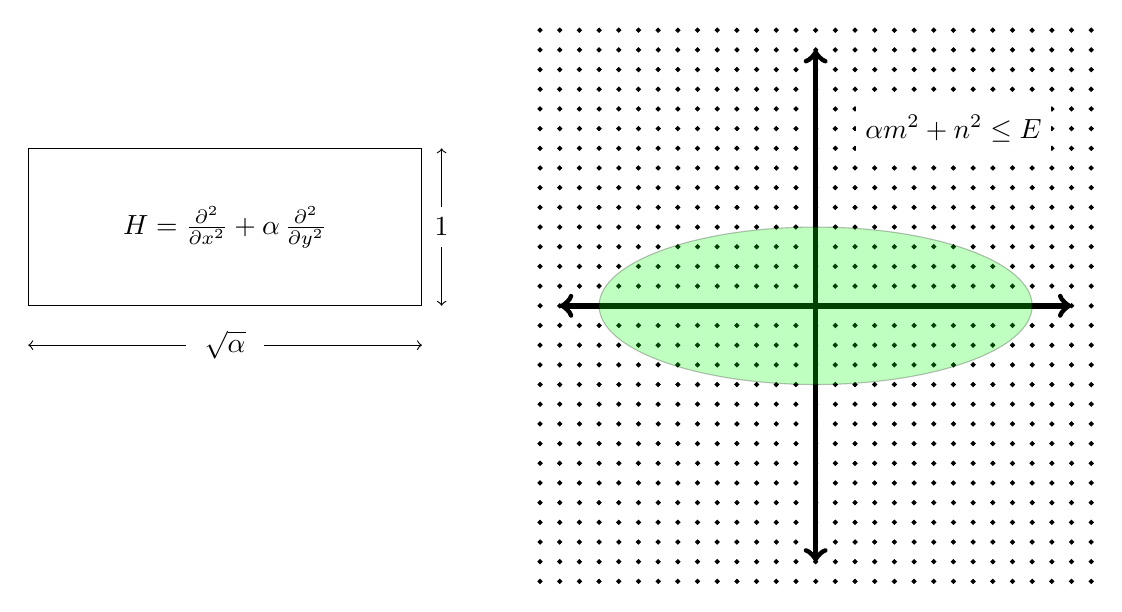
\begin{tikzpicture}

\begin{scope}

\node at (2.5,1) {$H = \frac{\partial^2}{\partial x^2}+ \alpha \, \frac{\partial^2}{\partial y^2} $};

\draw (0,0)--(5,0)--(5,2)--(0,2)--cycle;

\node at (2.5,-0.5) {$\sqrt{\alpha}$};
\draw[<-] (0,-0.5)--(2,-0.5);
\draw[->] (3,-0.5)--(5,-0.5);

\node at (5.25,1) {$1$};
\draw[->] (5.25,1.25)--(5.25,2);
\draw[<-] (5.25,0)--(5.25,0.75);

\end{scope}

\begin{scope}[xshift=10cm]

\draw[<->, line width=2] (-3.25,0)--(3.25,0);
\draw[<->, line width=2] (0,-3.25)--(0,3.25);

\foreach \a in {-3.5,-3.25,...,3.5}{
	\foreach \b in {-3.5,-3.25,...,3.5}{
	
		\draw[fill=black] (\a,\b) circle (0.025);
	}
}

\draw[fill=green, opacity=0.25] (0,0) circle [x radius = 2.75, y radius = 1];

\node[fill=white] at (1.75,2.25) {$\alpha m^2 + n^2 \leq E $}; 

\end{scope}

\end{tikzpicture} \\ \\
It is really at our discretion whether to read any further into the problem than this.  Weyl's theorem was a huge accomplishment in it's day and continues to yield results. \\ \\
We do continue. \\ \\
They want to know how much these numbers bunch together: 
$$ 1,\;\sqrt{2},\;  1 + \sqrt{2}, \; 4,\; 4 + \sqrt{2},\; 4 \sqrt{2},\; 1 + 4\sqrt{2}, \; 9, \;4 + 4 \sqrt{2}, \;\dots  $$
Bourgain branches off and on his own writes something about the ``Energy levels" associated to the free particle in a box.
$$
H = \frac{\partial^2}{\partial x^2}+ \alpha \, \frac{\partial^2}{\partial y^2}
+ \alpha \, \frac{\partial^2}{\partial z^2} \text{ and now } E = l^2 + \alpha \, m^2 + \beta \, n^2  $$
negative energy is OK.  In Quantum Mechanics, realistic systems have $E \geq 0$ ( I don't remember why). \\ \\
This seems like kid stuff and I don't know why this particular problem is important now.  On the other hand, it's one of the only few kind of problems I know how to do.

\newpage

\noindent Bourgain introduces these ``bumpfunctions" -- just use the step functions. 
$$w_1 = \left\{
\begin{array}{cc} 
1 &  \text{if }x \in [\frac{1}{2}, \frac{3}{4}]\\ \\
0 & \text{if }x \notin [\frac{1}{2}, \frac{3}{4}] \end{array}  \right. 
\hspace{0.25in}\text{and}\hspace{0.25in}
w_1 = \left\{
\begin{array}{cc} 
1 &  \text{if }x \in [-1,1]\\ \\
0 & \text{if }x \notin [-1,1]\end{array}  \right. $$
Forget it, I am just using step functions.  Maybe we'll regret this.  He's scared of this:
\begin{itemize}
\item in real life we have to truncate in physical space
\item and we have to truncate in Fourier space
\item therefore we overshoot and have extra copies of everything.
\end{itemize}
\includegraphics[width=3in]{oppenheim-03.png} \hspace{1in}
\includegraphics[width=3.25in]{oppenheim-04.png}
so even though we're trying to draw the thing straight, there are actually small slips everywhere.  With enough modes they do go away, but we do not have infinite resources so therefore tiny artifacts always exist. \\ \\
If you're a telephone company, all you care about are these tiny artifacts.  They become giants, as you customers start to complain about what they are hearing. \\ \\
Here's the real reason: {\color{blue!20!white} I never learned how smoothness differentability play out in the Fourier transform}.  Here's a good one:
\begin{quotation}
If $f \in L^1(\mathbb{T})$ is absolutely continuous then $\hat{f}(n) = O(n^{-1})$.
\end{quotation}
What about our step function?  $f(-0.0001) = 0$ and yet $f(+0.0001)=1$. Maybe our Fourier coefficients won't have this decay. 
$$ \hat{f}(n) = \int_0^1 e^{2\pi i \, n t} \, dt = \left\{ 
\begin{array}{cc}
1 & \text{if }n=0 \\ 
0 & \text{if }n\neq 0 \end{array} \right. $$
Well, our step functions $w_1$ live in $L^1(\mathbb{R})$ and not $L^1(\mathbb{T})$ (e.g. we only want one copy of our ``step", which is supposed to be smooth anyway).

\newpage

\noindent Even more problem:  I don't remember what \textbf{absolutely continuous}  actually meant.\footnote{I read much of 20th century Analsys and Topology as looking for shapes and sequences of numbers with increasingly ``bad" behavior.  And it's pretty dreaful.  But then maybe I thought, some of these pathologies are already happening and exist in nature.  And maybe what we think of a ``pathology" or a ``bad guy" can actually be quite helpful.  \\ Entropy is like that.  We think of change and randomness as pretty evil, but what if I called it ``fairness" or ``serendipity".  And there is mathematics of that.}  Continuous functions can be pretty weird. All Devil's staircase functions are continuous.  We can continuously map the unit interval into the entire square $[0,1] \to [0,1]^2$.  \\ \\
\includegraphics[width=3.25in]{oppenheim-05.jpg} \\ \\
Due to mistakes like these maybe I can read your e-mail or your Snapchat or Instagram direct messages.  And every know and then we hear of a hack. So if the phone company is constantly losing sleep over this, you and me, must be real suckers.
\\ \\ \\
By the way, I have that for functions with enough derivatives:
$$ \hat{f}(n) = o(n^{-k}) $$
Sometimes you cannot take the derivative, e.g. 
$$
f(x) = \left\{  \begin{array}{rc} 1 & x > 0 \\ -1 & x < 0\end{array}\right. $$
left of zero it's flat. right of zero it's flat.  What do we assign to $f'(0)$ ? \\
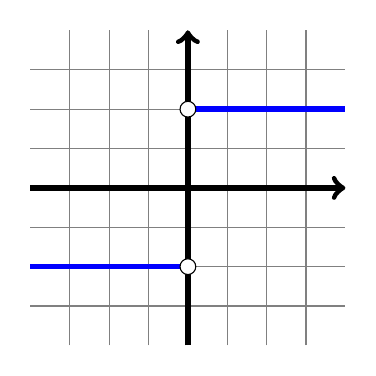
\begin{tikzpicture}[scale=0.5]
% notice how hard I am working to draw the coordinate grid.  maybe it's artificial?

\foreach \a  in {-3,...,3}{
	\draw[color=black!50!white] (-4,\a)--(4,\a);
	\draw[color=black!50!white] (\a,-4)--(\a,4);
}

\draw[line width =2, ->] (-4,0)--(4,0);
\draw[line width =2, ->] (0,-4)--(0,4);

\draw[color=blue, line width = 2] (-4,-2)--(0,-2);
\draw[color=blue, line width = 2] ( 0, 2)--(4, 2);

\draw[fill=white] (0, 2) circle (0.2);
\draw[fill=white] (0,-2) circle (0.2);

\end{tikzpicture}

\newpage 

\noindent We seek a lower bound for:
$$ \sum_{(x_1, x_2, x_3) \in \mathbb{Z}^3} 
w_1(\frac{x_1}{N})
w_1(\frac{x_2}{N})
w_1(\frac{x_3}{N}) \; \mathbf{1}_{\big\{|Q(x)-\xi| < N\big\}}
\approx \big\{|Q(x)-\xi| < N\big\} \cap \big\{ \frac{1}{2}N < x_1, x_2, x_3 < \frac{3}{4}N \big\}\cap \mathbb{Z}^3$$
The Bourgain's solo paper writes it on the left.  I have a much easier time with the version on the right.  Is obvious the next equation is the same as well?
$$ 
\big\{|\log(x_1^2 +\alpha_2 \, x_2^2 -\xi) - 2 \log x_3 - \log \alpha_3 | < \frac{\delta}{N^2} \big\} \cap \big\{ \frac{N}{2} < x_1, x_2, x_3 < \frac{3N}{4} \big\}\cap \mathbb{Z}^3 $$
and what was with the ridiculous range $[ \frac{1}{2}, \frac{3}{4}]$? 
\vspace{6pt}
\hrule
\vspace{6pt}
In Fourier space we can split things into ways that have no ``physical" counterpart.  Later we can ascribe them meaning, right now completely mysterious:
\begin{itemize}
\item $\displaystyle F_1(t) = \sum_{x_1, x_2 \in \mathbb{Z}} w_1(\frac{x_1}{N}) w_1(\frac{x_2}{N})
e^{it \; \log (x_1^2 +\alpha_2 \, x_2^2 -\xi)} = \sum_{x_1, x_2 \in \mathbb{Z}} \mathbf{1}\big(\tfrac{1}{2} < \tfrac{x_1}{N} , \tfrac{x_2}{N} < \tfrac{3}{4} \big)
(x_1^2 +\alpha_2 \, x_2^2 -\xi)^{it} $ \\
\item $F_2(t) = 
\sum_{x_1\in \mathbb{Z}} w_1(\frac{x_1}{N}) 
e^{it \; \log n} = \sum_{x_1\in \mathbb{Z}} \mathbf{1}\big(\tfrac{1}{2} < \tfrac{x_1}{N}  < \tfrac{3}{4} \big)
n^{it}
$
\end{itemize}
The simplified versions are mine.  Arguably, whenver I supply a detail that's not in Bourgain's I could turn it into an improvement on his estimates and that could be ``new" (in terms of academic-style research). \\ \\
I think he is writing ``Dirichlet series" the most famous one is the Riemann Zeta function:
$$ \zeta(it) = \sum n^{it} = 1^{it} + 2^{it} + 3^{it} + \dots $$
These truncations are all over the place.  It is the Fourier transform but the frequences are all log-scale, so 
$$ f \in \big\{ \log n : n \in \mathbb{Z} \big\} = \big\{ \log 1, \log 2, \log 3, \dots  \big\} $$
We're nearly done for the day.  
$$ \big\{|Q(x)-\xi| < N\big\} \cap \big\{ \frac{1}{2}N < x_1, x_2, x_3 < \frac{3}{4}N \big\}\cap \mathbb{Z}^3 \approx \frac{1}{T} \int_\mathbb{R} \widehat{w_2}(\frac{t}{T}) \, F_1(t) \overline{F_2(2t)}\,
e^{-it \log \alpha_3} \, dt $$
This is a good time to sit back and laugh.  This equation is going to be split as follows:
$$ (\ast) + (\ast \ast) := \widehat{w_2}(\frac{t}{\sqrt{N}})  + \big( \widehat{w_2}(\frac{t}{T})  - \widehat{w_2}(\frac{t}{\sqrt{N}}) \big) $$
Rather \dots we are going to split the Fourier transform this way:
\begin{itemize}
\item $(\ast) \;\;= \frac{1}{T} \int_\mathbb{R} \widehat{w_2}(\frac{t}{\sqrt{N}}) \, F_1(t) \overline{F_2(2t)}$
\item $(\ast \ast) = \frac{1}{T} \int_\mathbb{R} 
\Big(\widehat{w_2}(\frac{t}{T}) - \widehat{w_2}(\frac{t}{\sqrt{N}}) \Big)
 \, F_1(t) \overline{F_2(2t)}$
\end{itemize}
What did we just do?  I have no idea.  \\ \\
At least, we followed instruction as best we can.  Maybe it will be helpful to think of quantum mechanics and observables?  position and momentum space?  Could a signal-processing metaphor work?  There are brand new ideas, every day!

\newpage

\noindent \textbf{5/31} \dots 

\newpage

\begin{thebibliography}{}

\item J\'{a}nos Koll\'{a}r \textbf{Quadratic solutions of quadratic forms} \texttt{arXiv:1607.01276}

\item Ze\'{e}v Rudnick, Ezra Waxman  \textbf{Angles of Gaussian primes} \texttt{ arXiv:1705.07498}

\item Jean Bourgain. \textbf{A quantitative Oppenheim Theorem for generic diagonal quadratic forms} \texttt{arXiv:1604.02087}

\item Valentin Blomer, Jean Bourgain, Maksym Radziwi\l\l, Zeev Rudnick   \textbf{Small gaps in the spectrum of the rectangular billiard} \texttt{arXiv:1604.02413}


\end{thebibliography}



\vfill

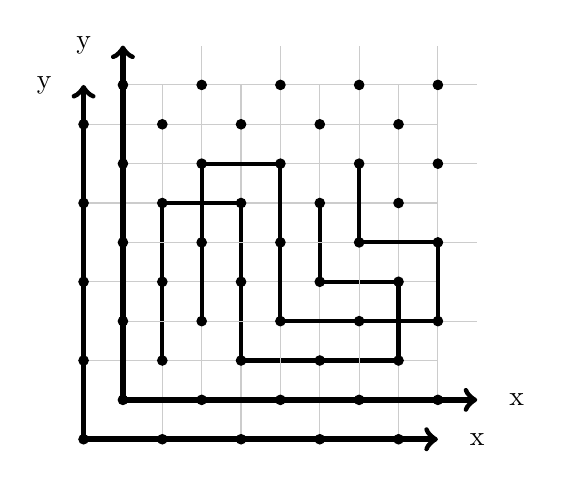
\begin{tikzpicture}

\node at ( 5,0) {x};
\node at (-0.5,4.5) {y};

\foreach \a in {0,...,4}{ 
	\draw[color=black!20!white] (\a,0)--(\a,4.5);
	\draw[color=black!20!white] (0,\a)--(4.5,\a);
 }

\draw[line width=2, ->] (0,0)--(4.5,0);
\draw[line width=2, ->] (0,0)--(0,4.5);

\foreach \a in {0,...,4}{
\foreach \x in {0,...,4}{
			\draw[fill=black] (\a,\x) circle (0.06);
	 }
}


\draw[line width=1.5] (1,1)--(1,2)--(1,3)--(2,3)--(2,1)--(4,1)--(4,2)--(3,2)--(3,3);


\begin{scope}[xshift=0.5cm, yshift=0.5cm]

\node at ( 5,0) {x};
\node at (-0.5,4.5) {y};

\foreach \a in {0,...,4}{ 
	\draw[color=black!20!white] (\a,0)--(\a,4.5);
	\draw[color=black!20!white] (0,\a)--(4.5,\a);
 }

\draw[line width=2, ->] (0,0)--(4.5,0);
\draw[line width=2, ->] (0,0)--(0,4.5);

\foreach \a in {0,...,4}{
\foreach \x in {0,...,4}{
			\draw[fill=black] (\a,\x) circle (0.06);
	 }
}


\draw[line width=1.5] (1,1)--(1,2)--(1,3)--(2,3)--(2,1)--(4,1)--(4,2)--(3,2)--(3,3);
\end{scope}


\end{tikzpicture}



\end{document}